\documentclass[11pt]{article}

\usepackage{amsmath, amssymb, amsthm}
\usepackage{mathtools}
\usepackage{tikz-cd}
\usetikzlibrary{calc, positioning, decorations.markings}
\usepackage{listings}
\usepackage{hyperref}
\usepackage[margin=1.2in]{geometry}

\newtheorem{theorem}{Theorem}[section]
\newtheorem{lemma}[theorem]{Lemma}
\newtheorem{proposition}[theorem]{Proposition}
\newtheorem{corollary}[theorem]{Corollary}
\newtheorem{definition}[theorem]{Definition}
\newtheorem{example}[theorem]{Example}
\newtheorem{remark}[theorem]{Remark}

\newcommand{\cat}[1]{\mathbf{#1}}
\newcommand{\Set}{\cat{Set}}
\newcommand{\Patch}{\mathcal{P}}
\newcommand{\tensor}{\otimes}
\newcommand{\comp}{\mathbin{;}}
\newcommand{\id}{\mathrm{id}}

\lstset{
    basicstyle=\ttfamily\small,
    columns=flexible,
    breaklines=true,
    frame=single,
    language=Java
}

\title{Infrastructure as Morphisms:\\A Categorical Semantics for Composable Resource Configuration}
\author{}
\date{}

\begin{document}
    \maketitle

    \begin{abstract}
        We present a categorical semantics for a framework in which infrastructure
        configuration is specified by composing typed morphisms in a symmetric monoidal
        category. Objects are multisets of typed ports; morphisms are \emph{boxes} that
        consume and produce resources along typed wires. Sequential composition connects
        outputs to inputs; the monoidal product places boxes in parallel. A partial
        commutative monoid of \emph{patches} governs how independent modifications to a
        shared entity combine. The resulting category is symmetric gs-monoidal with a
        partial comonoid structure.
        We prove that two programs produce identical output if and only if they are equal
        as morphisms, establish conditions under which composition order is irrelevant, and
        derive two practical consequences: mechanical migration between libraries of
        boxes, and decidable backwards-compatibility checking for box revisions.
    \end{abstract}

    \section{Introduction}

    Consider the problem of specifying a collection of named, persistent entities---each
    with a fixed \emph{type} drawn from a finite alphabet, a unique \emph{identity} (a
    string), and a \emph{property assignment} (a partial function from a type-determined
    set of paths to values)---together with directed references between them. We call such
    a specification a \emph{resource configuration}. It is the output artifact of what
    practitioners call \emph{Infrastructure-as-Code}: a declarative description of
    servers, databases, queues, access policies, and other cloud resources, written as a
    program that a deployment engine interprets.

    Concretely: a resource of type ``Queue'' might have properties \texttt{timeout} $= 60$
    and \texttt{retentionDays} $= 14$. A resource of type ``Function'' might have a property
    \texttt{role} whose value is a reference to the identity of a resource of type ``Role.''
    The deployment engine reads the full assignment for each identity and creates (or
    updates) the corresponding entity in the cloud environment.

    Existing frameworks represent programs as trees of mutable objects. Reorganising the
    tree changes the identities of the output entities, and no tractable equational theory
    exists for such programs. We propose an alternative: a configuration program is a
    morphism in a symmetric monoidal category $\cat{C}$. Objects are finite multisets of
    typed ports. Morphisms are functions (called \emph{boxes}) that consume resources along
    input wires and produce resources along output wires. Composition is wiring; the
    monoidal product is parallel juxtaposition.

    This view is an instance of the wiring diagram formalism of Fong and Spivak
    \cite{fong2019invitation}, specialised so that wires carry typed resources and boxes
    produce configuration patches. The key contribution is the identification of the
    \emph{patch monoid} (Section~\ref{sec:patch}) that governs how independent
    modifications combine, and the derivation from it of commutativity, confluence, and
    decidability results (Sections~\ref{sec:commutativity}--\ref{sec:compat}).

    \section{The Category $\cat{C}$}

    \subsection{Objects}

    Let $\Sigma$ be a countable set of \emph{type names}---labels such as
    $\mathsf{Queue}$, $\mathsf{Function}$, $\mathsf{Table}$, $\mathsf{Role}$. Each type
    name determines a finite set of property paths (its \emph{schema}).

    \begin{definition}
        The objects of $\cat{C}$ are the elements of the free commutative monoid
        $\mathbb{N}[\Sigma]$---that is, finite multisets over $\Sigma$. We write the
        monoidal product as $\tensor$ (multiset union) and the unit as $I$ (the empty
        multiset).
    \end{definition}

    We write $[A]$ for the singleton multiset, and $[A, B, C]$ for $\{A, B, C\}$. An
    object describes the \emph{interface} of a box: how many wires enter or leave, and
    what type each wire carries.

    \subsection{Morphisms}

    \begin{definition}\label{def:morphism}
        A morphism $f \colon X \to Y$ in $\cat{C}$ is a \emph{box}: a deterministic
        function that, given a tuple of resources whose types match $X$, produces a tuple
        whose types match $Y$. Each resource carries a \emph{logical identity} (a string
        that names it uniquely in the output configuration) and a \emph{property
        assignment} (a patch in the sense of Section~\ref{sec:patch}).
    \end{definition}

    Three important classes of morphisms arise:
    \begin{itemize}
        \item \emph{Constructors}: $I \to [A]$. Produce a fresh resource of type $A$
        with a chosen identity and initial properties.
        \item \emph{Transformers}: $[A] \to [A]$. Accept a resource on one wire and
        return it (same identity) with additional properties assigned.
        \item \emph{Wirers}: $[A, B] \to [A, B, C]$. Accept two resources, return them
        (possibly with added properties) together with a new auxiliary resource $C$ whose
        properties reference the first two.
    \end{itemize}

    \begin{example}\label{ex:three-boxes}
        Three boxes, drawn as string diagrams. Wires flow left to right. Each wire is
        labelled with the type it carries. A box with no input wires is a constructor; it
        produces a resource from nothing. A box whose output wires include its input wires
        (same type, same identity) is a transformer or wirer.

        \bigskip
        \begin{center}
        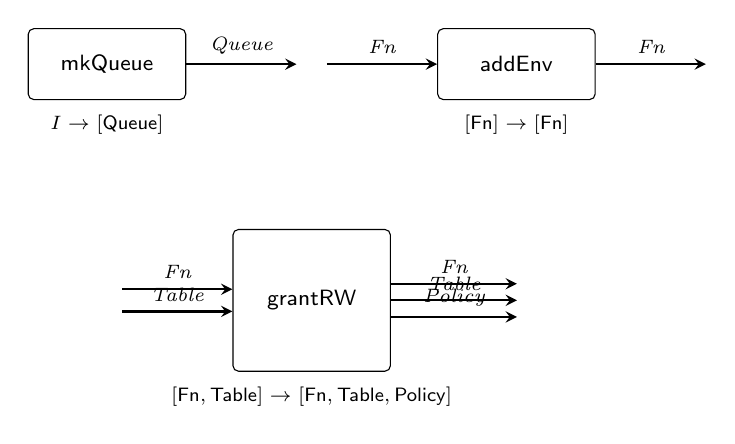
\begin{tikzpicture}[
            box/.style={draw, minimum width=2cm, minimum height=0.9cm,
                        rounded corners=2pt, font=\footnotesize\sffamily},
            arr/.style={-stealth, thick},
            lbl/.style={font=\scriptsize\itshape, above, midway}
        ]
        % --- Constructor: mkQueue ---
        \node[box] (mkq) at (0, 0) {mkQueue};
        \draw[arr] (mkq.east) -- ++(1.4,0) node[lbl] {Queue};
        \node[font=\scriptsize, below=2pt] at (mkq.south) {$I \to [\mathsf{Queue}]$};

        % --- Transformer: addEnv ---
        \node[box] (ae) at (5.2, 0) {addEnv};
        \draw[arr] ([xshift=-1.4cm]ae.west) -- (ae.west) node[lbl] {Fn};
        \draw[arr] (ae.east) -- ++(1.4,0) node[lbl] {Fn};
        \node[font=\scriptsize, below=2pt] at (ae.south) {$[\mathsf{Fn}] \to [\mathsf{Fn}]$};

        % --- Wirer: grantRW ---
        \node[box, minimum height=1.8cm] (gr) at (2.6, -3) {grantRW};
        % inputs
        \draw[arr] ([xshift=-1.4cm, yshift=4pt]gr.west) -- ([yshift=4pt]gr.west)
            node[lbl] {Fn};
        \draw[arr] ([xshift=-1.4cm, yshift=-4pt]gr.west) -- ([yshift=-4pt]gr.west)
            node[lbl] {Table};
        % outputs
        \draw[arr] ([yshift=6pt]gr.east) -- ++(1.6,0) node[lbl] {Fn};
        \draw[arr] (gr.east) -- ++(1.6,0) node[lbl] {Table};
        \draw[arr] ([yshift=-6pt]gr.east) -- ++(1.6,0) node[lbl] {Policy};
        \node[font=\scriptsize, below=2pt] at (gr.south)
            {$[\mathsf{Fn},\mathsf{Table}] \to [\mathsf{Fn},\mathsf{Table},\mathsf{Policy}]$};
        \end{tikzpicture}
        \end{center}
        \bigskip

        The constructor \emph{mkQueue} takes no input and produces a Queue on its single
        output wire. The transformer \emph{addEnv} receives a Function and returns it with
        an additional property set. The wirer \emph{grantRW} receives a Function and a
        Table, passes both through (adding a property to the Function's associated Role),
        and emits a new Policy resource whose properties reference both inputs.
    \end{example}

    \begin{remark}[Wires carry more than types]
        The type system of $\cat{C}$ tracks only resource types on wires, but the
        \emph{values} flowing on wires are richer: each resource carries its identity and
        full property assignment. Boxes may also accept and produce scalar values (strings,
        numbers, arrays) as parameters---these appear in the implementation as ordinary
        function arguments but do not correspond to wires in the categorical sense. A wire
        represents a \emph{resource with identity and persistent state}; a scalar parameter
        is a pure value with no corresponding entity in the output configuration.
    \end{remark}

    \subsection{Composition}

    Sequential composition $f \comp g$ is defined when the output type of $f$ equals the
    input type of $g$. The output resources of $f$ become the input resources of $g$,
    matched by position and type.

    The monoidal product $f \tensor g$ runs $f$ and $g$ on disjoint resource sets and
    concatenates their outputs.

    \subsection{Monoidal structure}

    \begin{proposition}
        $(\cat{C}, \tensor, I)$ is a strict symmetric monoidal category.
    \end{proposition}

    \begin{proof}
        Objects are multisets; multiset union is strictly associative with the empty multiset
        as unit. The braiding $\sigma_{X,Y} \colon X \tensor Y \to Y \tensor X$ permutes
        the resource tuple. Naturality and symmetry ($\sigma_{Y,X} \circ \sigma_{X,Y} =
        \id_{X \tensor Y}$) follow from commutativity of multiset union.
    \end{proof}

    \subsection{Comonoid structure}

    Every object $X$ carries a cocommutative comonoid:
    \begin{itemize}
        \item Comultiplication $\Delta_X \colon X \to X \tensor X$ (the same resource
        appears on two output wires---it is ``shared'').
        \item Counit $\varepsilon_X \colon X \to I$ (the resource is removed from the
        output configuration entirely---it is ``discarded'').
    \end{itemize}

    The comonoid laws hold. This makes $\cat{C}$ a \emph{gs-monoidal category}
    \cite{gadducci1997inductive}---``gs'' for garbage (discard) and sharing (copy).

    The comonoid structure is \emph{partial}: the composition $\Delta_X \comp (f \tensor g)$,
    which copies a resource and modifies the two copies independently, is well-defined only
    when the patches produced by $f$ and $g$ are \emph{compatible}---a notion made precise
    in the next section.

    \section{The Patch Monoid}
    \label{sec:patch}

    \subsection{Patches as partial functions}

    Fix a type $A \in \Sigma$. Its schema determines a finite set $\Pi_A$ of property
    paths. A \emph{patch} for $A$ is a partial function $p \colon \Pi_A \rightharpoonup V$
    (where $V$ is an appropriate value domain).

    \begin{definition}\label{def:patch-merge}
        Let $\Patch_A$ denote the set of patches for type $A$. Define a partial binary
        operation $\cdot$ on $\Patch_A$: for patches $p, q$ and each path $\pi \in \Pi_A$,
        \[
            (p \cdot q)(\pi) =
            \begin{cases}
                p(\pi) & \text{if } \pi \in \mathrm{dom}(p) \setminus \mathrm{dom}(q), \\
                q(\pi) & \text{if } \pi \in \mathrm{dom}(q) \setminus \mathrm{dom}(p), \\
                p(\pi) & \text{if } \pi \in \mathrm{dom}(p) \cap \mathrm{dom}(q)
                          \text{ and } p(\pi) = q(\pi), \\
                \bot   & \text{if } \pi \in \mathrm{dom}(p) \cap \mathrm{dom}(q)
                          \text{ and } p(\pi) \neq q(\pi).
            \end{cases}
        \]
        The merge $p \cdot q$ is \emph{defined} if and only if $\bot$ does not arise at
        any path. We say $p$ and $q$ are \emph{compatible} when $p \cdot q$ is defined.
        The identity element is the empty patch $\emptyset$ (the totally undefined partial
        function).
    \end{definition}

    \begin{proposition}\label{prop:pcm}
        $(\Patch_A, \cdot, \emptyset)$ is a partial commutative monoid.
    \end{proposition}

    \begin{proof}
        Commutativity: the case analysis in Definition~\ref{def:patch-merge} is symmetric
        in $p$ and $q$. Associativity: at each path $\pi$, the result of $(p \cdot q)
        \cdot r$ and $p \cdot (q \cdot r)$ is the unique value assigned by whichever
        patches define $\pi$, or $\bot$ if two distinct values appear---independent of
        grouping. Unitality: $\emptyset$ assigns no paths, so $p \cdot \emptyset = p$.
    \end{proof}

    \subsection{The synthesis function}

    A program---a composite morphism $P$ in $\cat{C}$---produces a finite collection of
    resources in its output configuration. Each resource is identified by a logical
    identity $\ell$ (a unique string) and assembled from patches: each box in the
    composition that touches $\ell$ contributes a patch to it.

    \begin{definition}
        Let $P$ be a program. For each logical identity $\ell$ produced by $P$, let
        $p_1, \ldots, p_n \in \Patch_{A_\ell}$ be the patches contributed to $\ell$ by
        the boxes in $P$. The \emph{synthesis} of $P$ is the partial function
        \[
            \mathrm{synth}(P) \colon \ell \mapsto p_1 \cdot p_2 \cdot \ldots \cdot p_n
        \]
        defined on the set of identities produced by $P$. By Proposition~\ref{prop:pcm},
        the merge order and bracketing are irrelevant.
    \end{definition}

    \begin{definition}
        A program $P$ is \emph{valid} if $\mathrm{synth}(P)(\ell)$ is defined (no
        conflicts) for every identity $\ell$ in its domain.
    \end{definition}

    The output of a valid program is a finite map from identities to patches, together
    with a type assignment $\ell \mapsto A_\ell$. This is the resource configuration.
    Observe that the entire program---regardless of how deeply nested its boxes
    are---reduces to a single morphism $I \to [A_1, \ldots, A_k]$ whose output is exactly
    this configuration. The program \emph{is} a box, from nothing to a multiset of typed
    resources.

    \section{Commutativity of Independent Boxes}
    \label{sec:commutativity}

    \begin{definition}
        Two transformers $f, g \colon [A] \to [A]$ are \emph{independent} if their patches
        $p_f, p_g$ have disjoint domains: $\mathrm{dom}(p_f) \cap \mathrm{dom}(p_g) =
        \emptyset$.
    \end{definition}

    \begin{theorem}[Commutativity]\label{thm:commute}
        If $f$ and $g$ are independent, then $f \comp g = g \comp f$ in $\cat{C}$.
    \end{theorem}

    \begin{proof}
        Both sides produce the patch $p_f \cdot p_g$ for the shared identity. Disjoint
        domains imply compatibility ($p_f \cdot p_g$ is always defined). Commutativity of
        $\cdot$ (Proposition~\ref{prop:pcm}) gives $p_f \cdot p_g = p_g \cdot p_f$.
        Since the identity and type are unchanged by either composition, the output
        resources are identical.
    \end{proof}

    \begin{corollary}[Confluence]\label{cor:confluence}
        If $f_1, \ldots, f_n \colon [A] \to [A]$ are pairwise independent, then any
        permutation of their sequential composition yields the same morphism.
    \end{corollary}

    \begin{proof}
        Adjacent independent pairs commute by Theorem~\ref{thm:commute}; any two
        permutations are related by a sequence of such transpositions.
    \end{proof}

    \begin{example}\label{ex:commute}
        Two different orderings of independent wirers, drawn as string diagrams. Both
        produce identical output.

        \bigskip
        \begin{center}
        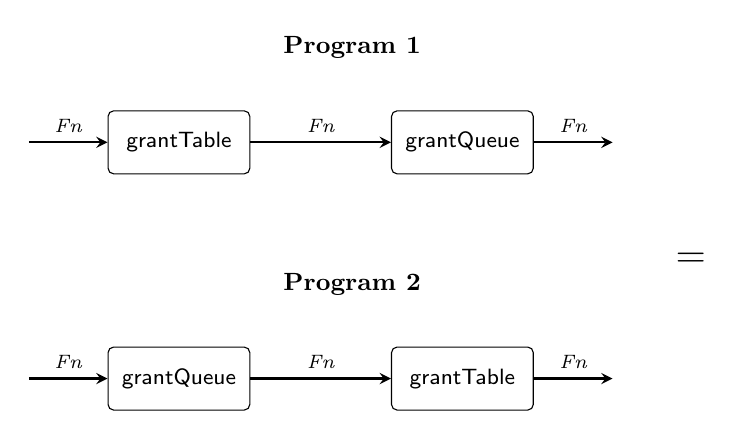
\begin{tikzpicture}[
            box/.style={draw, minimum width=1.8cm, minimum height=0.8cm,
                        rounded corners=2pt, font=\footnotesize\sffamily},
            arr/.style={-stealth, thick},
            lbl/.style={font=\scriptsize\itshape, above, midway}
        ]
        % Program 1: grantTable then grantQueue
        \node[font=\small\bfseries] at (2.2, 1.2) {Program 1};
        \node[box] (gt1) at (0, 0) {grantTable};
        \node[box] (gq1) at (3.6, 0) {grantQueue};
        \draw[arr] ([xshift=-1cm]gt1.west) -- (gt1.west) node[lbl] {Fn};
        \draw[arr] (gt1.east) -- (gq1.west) node[lbl] {Fn};
        \draw[arr] (gq1.east) -- ++(1cm, 0) node[lbl] {Fn};

        % Program 2: grantQueue then grantTable
        \node[font=\small\bfseries] at (2.2, -1.8) {Program 2};
        \node[box] (gq2) at (0, -3) {grantQueue};
        \node[box] (gt2) at (3.6, -3) {grantTable};
        \draw[arr] ([xshift=-1cm]gq2.west) -- (gq2.west) node[lbl] {Fn};
        \draw[arr] (gq2.east) -- (gt2.west) node[lbl] {Fn};
        \draw[arr] (gt2.east) -- ++(1cm, 0) node[lbl] {Fn};

        % Equals sign
        \node[font=\Large] at (6.5, -1.5) {$=$};
        \end{tikzpicture}
        \end{center}
        \bigskip

        The box \emph{grantTable} assigns properties at paths beneath
        \texttt{role.tablePolicy}; the box \emph{grantQueue} assigns properties at paths
        beneath \texttt{role.queuePolicy}.\footnote{These path names are
        schematic. In the concrete system that motivates this work, each box creates a
        separate auxiliary resource (an access policy) rather than writing to distinct
        sub-paths of a single resource. The disjointness that enables commutativity holds
        at the level of logical identities: each box contributes patches to resources the
        other does not touch.} These paths are disjoint, so the patches are compatible
        regardless of order. The commutativity theorem guarantees that the two programs
        denote the same morphism.
    \end{example}

    \section{String Diagrams and Faithfulness}

    Every morphism in a symmetric monoidal category admits a string diagram representation
    \cite{joyal1991geometry, selinger2010survey}. In $\cat{C}$:

    \begin{itemize}
        \item Wires are lines labelled by types from $\Sigma$.
        \item Boxes are labelled nodes with input ports (left) and output ports (right).
        \item $\tensor$ is vertical juxtaposition.
        \item $\comp$ is horizontal connection of matching ports.
        \item $\sigma$ is a wire crossing.
        \item $\Delta$ is a wire fork (one wire becomes two).
        \item $\varepsilon$ is a wire cap (termination).
    \end{itemize}

    \begin{theorem}[Faithfulness of string diagrams]\label{thm:faithful}
        Two string diagrams represent the same morphism in $\cat{C}$ if and only if they
        are related by planar isotopy.
    \end{theorem}

    \begin{proof}
        This is the coherence theorem for symmetric monoidal categories
        \cite{joyal1991geometry}. $\cat{C}$ satisfies the hypotheses: strict monoidal
        structure and symmetric braiding.
    \end{proof}

    A consequence: any graphical interface that renders a program as a string diagram may
    freely rearrange box positions without changing the program's denotation, provided the
    wiring topology is preserved.

    \section{Nesting and the Operadic Perspective}
    \label{sec:operad}

    \subsection{What nesting means}

    A box $h \colon X \to Y$ may be defined as a composition of smaller boxes $f$ and $g$
    internally. In the monoidal category, $h$ is simply the composite morphism $h = f
    \comp g$ (or a more complex wiring involving $\tensor$, $\sigma$, $\Delta$). From the
    category's viewpoint, $h$ is indistinguishable from any other morphism $X \to Y$ with
    the same denotation.

    But a user benefits from retaining the \emph{decomposition}---knowing that $h$ is
    built from $f$ and $g$, and being able to ``zoom in'' to see how. This is extra
    structure not captured by the category alone.

    \subsection{The operad of wiring diagrams}

    Fong and Spivak \cite[Chapter~2]{fong2019invitation} formalise this as an
    \emph{operad} $\mathcal{W}$ of wiring diagrams. An operad captures
    \emph{substitution}: given a box with typed ports, one can fill it with an arrangement
    of smaller boxes whose collective external interface matches the outer box's interior
    interface. The operad's composition operation is this filling.

    In our framework:
    \begin{itemize}
        \item An element of $\mathcal{W}$ is a box together with a specification of how
        its internal wires are routed between sub-boxes.
        \item Operadic composition corresponds to defining a composite box in terms of
        previously defined ones.
        \item The operad retains the nesting hierarchy; the category forgets it.
    \end{itemize}

    \subsection{Relationship between the two views}

    There is a forgetful functor from the operad (nested diagrams) to the category (flat
    morphisms): it evaluates the composition, discarding the internal structure. Two
    operadic terms that map to the same morphism under this functor are
    \emph{observationally equivalent}---they produce the same output configuration.

    This is the formal content of the re-presentation theorem below
    (Section~\ref{sec:repr}): different nestings of the same underlying boxes can denote
    the same flat morphism. The nesting is a \emph{presentation} choice, not a semantic
    distinction.

    \subsection{What operads add}

    The operadic structure provides:
    \begin{enumerate}
        \item \emph{Hierarchical abstraction.} A user defines a composite box once and
        reuses it without thinking about its internals.
        \item \emph{Zoom.} A graphical interface can expand or collapse composite boxes,
        showing more or less detail.
        \item \emph{Provenance.} When two programs are observationally equivalent but
        structured differently, the operadic decomposition records \emph{why}---which
        sub-boxes were used, in what arrangement.
    \end{enumerate}

    The category $\cat{C}$ provides the equational theory (when are two programs the
    same?). The operad $\mathcal{W}$ provides the structural theory (how is a program
    built up from parts?). Both are needed: the first for correctness reasoning, the
    second for human comprehension.

    \section{Re-Presentation and Mechanical Migration}
    \label{sec:repr}

    \subsection{The practical problem}

    A programmer writes a configuration using one library of boxes $L$ (a set of named,
    reusable morphisms). Later, they wish to migrate to a different library $L'$---perhaps
    because $L'$ offers better abstractions, or because $L$ is deprecated, or because a
    team convention changed. The question: can the migration be performed mechanically,
    with a guarantee that the output configuration is unchanged?

    \subsection{Programs as words}

    A \emph{library} is a finite set $L = \{b_1, \ldots, b_n\}$ of boxes. A program over
    $L$ is a composite of elements from $L$, braiding, $\Delta$, and $\varepsilon$. Two
    different libraries $L$ and $L'$ may generate overlapping subcategories of $\cat{C}$.

    \begin{definition}
        The \emph{re-presentation problem}: given a valid program $P$ over $L$ and a
        target library $L'$, find a valid program $Q$ over $L'$ such that $P = Q$ in
        $\cat{C}$.
    \end{definition}

    This is the algebraic \emph{re-presentation problem}: given two generating sets of a
    common structure, translate a word from one to the other.

    \subsection{Decidability}

    We restrict attention to \emph{terminating} boxes: boxes that halt on every input.
    This is an assumption on the morphisms of $\cat{C}$, not a consequence of its
    structure. All boxes built by finite composition of property assignments and
    conditionals over finite schemas satisfy this assumption; boxes containing arbitrary
    recursion may not.

    \begin{theorem}[Decidability of equivalence]\label{thm:decide}
        For any two valid programs $P$ and $Q$ in $\cat{C}$ composed of terminating
        boxes, and sharing the same closed inputs (no free resource variables), the
        question ``$P = Q$?'' is decidable.
    \end{theorem}

    \begin{proof}
        Execute both programs: apply each box in sequence, collect the patches, merge them
        per identity, and produce the output map. Both executions terminate (by
        assumption). The outputs are finite maps; equality of finite maps is decidable.
    \end{proof}

    \begin{remark}
        The word problem for finitely presented categories is undecidable in general.
        Decidability here rests on two conditions: termination of all boxes, and the
        existence of a computable normal form (the synthesised output).
    \end{remark}

    \subsection{Tractability}

    Decidability of equivalence means we can \emph{verify} a candidate re-presentation.
    \emph{Finding} one requires search. The search is constrained by:

    \begin{enumerate}
        \item \emph{Per-identity decomposition.} The output decomposes as one patch per
        identity. The re-presentation decomposes likewise: for each identity, find a
        sub-composition in $L'$ that produces the same patch.
        \item \emph{Finite characterisation of boxes.} Each box in $L'$ can be run on
        representative inputs to observe its patch contribution. This fingerprint is
        finite and computable.
        \item \emph{Small patterns.} Boxes in $L'$ typically compose 3--10 primitive
        operations. The subgraph patterns to match are small.
    \end{enumerate}

    The practical algorithm is subgraph matching on the wiring diagram, with soundness
    verified by Theorem~\ref{thm:decide}.

    \section{Backwards Compatibility}
    \label{sec:compat}

    \subsection{Formulation}

    A library author publishes box $f \colon X \to Y$. Users incorporate $f$ into their
    programs. The author revises $f$ to $f'$ (same type). The question: can users adopt
    $f'$ without changing their output configuration?

    \begin{definition}
        $f'$ is \emph{strictly compatible} with $f$ if for all inputs $a$ of type $X$,
        $\mathrm{synth}(f'(a)) = \mathrm{synth}(f(a))$.
    \end{definition}

    \begin{definition}
        $f'$ is \emph{patch-compatible} with $f$ if for all inputs $a$ and every identity
        $\ell$, every path assigned by $f(a)$ is assigned by $f'(a)$ to the same value:
        $\mathrm{patches}(f(a)) \sqsubseteq \mathrm{patches}(f'(a))$, where $\sqsubseteq$
        is the sub-function ordering.
    \end{definition}

    Patch-compatibility allows $f'$ to assign \emph{additional} properties (additive
    change) but forbids removing or altering existing ones.

    \subsection{Compositionality of compatibility}

    \begin{proposition}\label{prop:compose-compat}
        Let $L = \{f_1, \ldots, f_n\}$ and $L' = \{f'_1, \ldots, f'_n\}$ be two versions
        of a library, with each $f'_i$ patch-compatible with $f_i$. Then for any valid
        program $P$ over $L$, the corresponding program $P'$ (obtained by replacing each
        $f_i$ with $f'_i$) satisfies $\mathrm{patches}(P) \sqsubseteq \mathrm{patches}(P')$.
    \end{proposition}

    \begin{proof}
        The output patches of $P$ are merges of patches contributed by the $f_i$.
        Replacing $f_i$ with $f'_i$ preserves every path-value assignment (by
        patch-compatibility) and may add new ones. Since $\sqsubseteq$ is preserved under
        $\cdot$ (if $p \sqsubseteq p'$ and $q \sqsubseteq q'$ and $p' \cdot q'$ is
        defined, then $p \cdot q$ is defined and $p \cdot q \sqsubseteq p' \cdot q'$),
        the merged output of $P'$ is a super-assignment of that of $P$.
    \end{proof}

    \begin{remark}
        Strict compatibility composes trivially: if each $f'_i$ produces identical patches
        to $f_i$, the merged output is unchanged. Patch-compatibility requires the
        additional observation that additive patches to fresh identities cannot conflict
        with pre-existing ones, and that the sub-function ordering is preserved by the
        merge operation.
    \end{remark}

    \subsection{Checking compatibility in practice}

    Compatibility is universally quantified over inputs. Since boxes may accept scalar
    parameters (strings, numbers) drawn from infinite domains, and their output may depend
    on these values, compatibility is \emph{not} decidable in general---it reduces to
    checking equivalence of arbitrary functions.

    \begin{theorem}\label{thm:compat}
        Strict and patch compatibility are decidable for the class of \emph{structurally
        determined} boxes: boxes whose patch contribution depends only on the types and
        identities of their resource inputs, not on scalar parameter values.
    \end{theorem}

    \begin{proof}
        For a structurally determined box $f \colon X \to Y$, the input type $X$ fixes
        the resource types and their reference topology. The space of structurally distinct
        inputs (varying only identity strings and reference presence) is finite. Execute
        both versions on each structural case and compare outputs (which is decidable for
        closed programs by Theorem~\ref{thm:decide}).
    \end{proof}

    For boxes that branch on scalar values, compatibility cannot be decided in finite
    time. However, the framework's properties---purity (no hidden state), observability
    (the output of any single execution is a finite, inspectable map), and termination
    (for well-behaved boxes)---make compatibility \emph{effectively testable}. A
    property-based testing approach generates random inputs from the type schema and checks
    the compatibility predicate on each. Any counterexample found is genuine (purity
    ensures reproducibility). Absence of counterexamples does not constitute a proof, but
    provides confidence proportional to coverage of the input space.

    \section{Relation to Prior Work}

    Fong and Spivak \cite{fong2019invitation} introduce wiring diagrams in two settings:
    as an operad (Chapter~2, nesting) and as symmetric monoidal preorders (Chapter~4,
    resource convertibility). Our category is richer than a preorder---it has many
    morphisms between the same pair of objects---and richer than a bare operad---it carries
    the patch monoid that governs merging.

    The gs-monoidal structure was introduced by Gadducci and Heckel
    \cite{gadducci1997inductive} and developed by Corradini and Gadducci
    \cite{corradini1999algebraic}. Our partial comonoid adds a compatibility constraint:
    sharing is well-defined only when downstream modifications merge without conflict.

    The use of string diagrams as a programming syntax follows Bonchi, Soboci\'{n}ski,
    and Zanasi \cite{bonchi2017interacting}, who establish soundness and completeness for
    symmetric monoidal categories.

    Partial commutative monoids appear in concurrency theory (e.g.\ trace monoids
    \cite{diekert1995book}) where independent actions commute. Our patch monoid is an
    instance: independent property assignments are the ``independent letters'' whose
    order is irrelevant.

    \section{Conclusion}

    We have exhibited a symmetric monoidal category whose morphisms are infrastructure
    configuration programs. The partial commutative monoid of patches captures the merge
    semantics of parallel modification. The key results:

    \begin{enumerate}
        \item Equivalence of closed programs is decidable (Theorem~\ref{thm:decide}).
        \item Independent transformers commute (Theorem~\ref{thm:commute}).
        \item Patch-compatibility composes across libraries
            (Proposition~\ref{prop:compose-compat}).
        \item Backwards compatibility is decidable for structurally determined boxes,
            and effectively testable in general (Theorem~\ref{thm:compat}).
    \end{enumerate}

    These rest on two properties: \emph{purity} (a box's meaning is its patch
    contribution) and \emph{observable normal form} (every program has a computable
    canonical output). Together they yield an effective equational theory, enabling
    mechanical refactoring, automated migration, and regression detection as decidable
    problems rather than heuristics.

    \begin{thebibliography}{9}

        \bibitem{fong2019invitation}
        B.~Fong and D.I.~Spivak,
        \emph{An Invitation to Applied Category Theory: Seven Sketches in Compositionality},
        Cambridge University Press, 2019.

        \bibitem{gadducci1997inductive}
        F.~Gadducci and R.~Heckel,
        ``An inductive view of graph transformation,''
        \emph{Recent Trends in Algebraic Development Techniques}, LNCS 1376, Springer,
        1997, pp.~223--237.

        \bibitem{corradini1999algebraic}
        A.~Corradini and F.~Gadducci,
        ``An algebraic presentation of term graphs, via gs-monoidal categories,''
        \emph{Applied Categorical Structures}, vol.~7, pp.~299--331, 1999.

        \bibitem{joyal1991geometry}
        A.~Joyal and R.~Street,
        ``The geometry of tensor calculus, I,''
        \emph{Advances in Mathematics}, vol.~88, no.~1, pp.~55--112, 1991.

        \bibitem{selinger2010survey}
        P.~Selinger,
        ``A survey of graphical languages for monoidal categories,''
        \emph{New Structures for Physics}, Lecture Notes in Physics, vol.~813, Springer,
        2010, pp.~289--355.

        \bibitem{bonchi2017interacting}
        F.~Bonchi, P.~Soboci\'{n}ski, and F.~Zanasi,
        ``Interacting Hopf algebras,''
        \emph{Journal of Pure and Applied Algebra}, vol.~221, no.~1, pp.~144--184, 2017.

        \bibitem{diekert1995book}
        V.~Diekert and G.~Rozenberg, eds.,
        \emph{The Book of Traces},
        World Scientific, 1995.

    \end{thebibliography}

\end{document}
